\chapter{The $N$-representability problem}\label{ch2}

For a given wave function, the \gls{2dm} can be calculated using its definition. However, when given a random symmetric matrix,
is it possible to find a corresponding (ensemble of) wave function which has the given matrix as the \gls{2dm}? This is the essence of the $N$-representability problem.

\section{General \mbox{$N$-representability} theorem}\label{ch2-general-n-rep}
A graphical depiction of this theorem can be found in \Vref{ch2-fig1}. The boundary of the convex set
of $N$-representable $p$th-order reduced density matrices is formed by an infinite number of tangent hyperplanes, where
each hyperplane represents a $p$-particle Hamiltonian and its ground state energy.
\begin{figure}
    \centering
    
\includegraphics[width=\textwidth]{n-representability}
    \caption{Graphical depiction of the necessary and sufficient conditions for $N$-representability. Every Hamiltonian $H^{(p)}$ can be represented by a hyperplane that bounds the convex set of $N$-representable ${^p\Gamma}$.}
    \label{ch2-fig1}
\end{figure}

\section{Approximately $N$-representability conditions}\label{2-approx-n-representability}
In \Vref{ch2-general-n-rep} we showed the necessary and sufficient conditions for $N$-representability. These required the knowledge of the
ground state energy of every possible Hamiltonian and are thus not usable as a sufficient condition. We can, however, use it as a necessary
condition: if we restrict XX to Hamiltonians of which we know the ground state energy or a lower bound on it, we can approximate the convex set of $N$-representable \gls{2dm}'s.
\begin{figure}
    \centering
    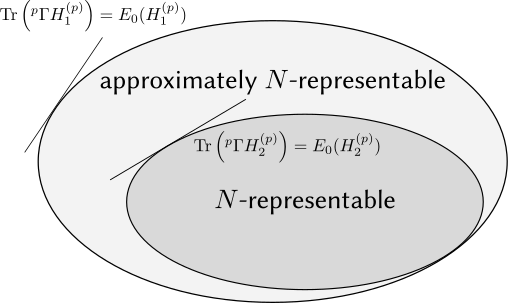
\includegraphics[width=0.9\textwidth]{approx-n-representability}
    \caption{Graphical depiction of the necessary conditions for $N$-representability. $H_1^{(p)}$ belongs to the class of Hamiltonians of which we know a bound on ground state energy while $H_2^{(p)}$ does not. The true convex set of $N$-representable ${^p\Gamma}$ is smaller than the approximate convex set delimited by the Hamiltonians of the class of $H_1^{(p)}$.}
    \label{ch2-fig3}
\end{figure}
In \Vref{ch2-fig3} we give a graphical interpretation of this idea. The approximate set of $N$-representable \gls{2dm} will be larger than the true set: there will be \gls{2dm}'s which fulfil all the necessary conditions but are still not derivable from an ensemble of wave functions.
As a consequence the variational optimization of the \gls{2dm} will give a lower bound on the energy. This is one of the highly attractive features of \gls{v2dm}.

\section{Symmetry considerations}\label{ch2-sym}

\subsection{Spatial point group symmetry}\label{ch2-pointsym}

For example, the $\ce{C2H4}$ molecule shown in \Vref{2-fig4} has $D_{2h}$ symmetry.
\begin{figure}[h]
    \centering
    \chemfig{H-[1]C(-[3]H)=C(-[1]H)(-[:-45]H)}
    \caption{The ethylene molecule has $D_{2h}$ symmetry.}
    \label{2-fig4}
\end{figure}
The main two-fold rotation axis is the connecting axis between the two carbon atoms (the z-axis). The two two-fold rotation axes are the x- and y-axis. The three reflection planes are xy, xz and yz.

As an example, we show the character table and the multiplication table of $C_{2}$ group in \Vref{2-tab1}.
\begin{table}
    \begin{subtable}{.5\linewidth}
        \centering
        \begin{tabular}{c|cc}
            & $E$ & $C_2$ \\
            \hline
            A & 1 & 1 \\
            B & 1 & -1
        \end{tabular}
        \caption{Character table of $C_2$}
        \label{2-tab1a}
    \end{subtable}
    ~
    \begin{subtable}{.5\linewidth}
    \centering
    \begin{tabular}{c|cc}
        & A & B \\
        \hline
        A & A & B \\
        B & B & A 
    \end{tabular}
    \caption{Multiplication table of $C_2$}
    \label{2-tab1b}
    \end{subtable}
    \caption{$C_2$ overview: it has 2 classes of operations. The identity operation and rotations over $180\degree$. The two irreducible representations are $A$ and $B$.}
    \label{2-tab1}
\end{table}
The character table contains the trace of the matrices of the irreducible representations. It it split up into conjugacy classes as the trace is invariant under a similarity transformation. These tables are extremely useful for decomposing a representation in its irreducible parts. The first irreducible representation $A$ is called the trivial representation because all the representation matrices (scalars in this case) are one. Every group has this irreducible representation.

\section{The doubly-occupied Hilbert space}\label{ch2-doci}
In previous sections, we only made general assumptions about the (ensemble of) wave functions from which the \gls{2dm} is derivable. All wave functions should be normalized and antisymmetric. For symmetry, we made assumptions on the quantum numbers of the wave function: it should be a singlet wave function, or the wave function should transform according to a certain irreducible representation.
But we could make other or additional assumptions. If we take a look at the \acrfull{fullci} expansion of the wave function, we see that a Slater determinant is the basic building block
\begin{equation}
    \ket{\Psi} = \sum_\mathbf{k} \sum_\mathbf{s} c_{\mathbf{k};\mathbf{s}} ~ \padd{k_1 s_1}\padd{k_2s_2}\ldots\padd{k_Ns_N}\ket{},
        \label{2-eq106}
\end{equation}

% vim: spell spelllang=en syntax=tex  tw=140
